\documentclass[10pt]{article}
% Shared preamble for the Apart sprint papers (layout follows the official template).
% Usage: % Shared preamble for the Apart sprint papers (layout follows the official template).
% Usage: % Shared preamble for the Apart sprint papers (layout follows the official template).
% Usage: \input{../apart_preamble.tex}  after \documentclass[11pt]{article}
\usepackage[T1]{fontenc}
\usepackage[utf8]{inputenc}
\usepackage{lmodern}          % only Latin Modern is installed for pdflatex here
\usepackage[letterpaper,margin=1in]{geometry}
\usepackage{amsmath,amssymb}
\usepackage{graphicx}
\usepackage{booktabs,array,tabularx}
\usepackage[usenames]{xcolor}
\usepackage[font=small,labelfont=bf,labelsep=period,justification=justified,singlelinecheck=false]{caption}
\usepackage[authoryear,round]{natbib}
\usepackage{url}
\usepackage[colorlinks=true,linkcolor=blue!50!black,citecolor=blue!50!black,urlcolor=blue!50!black]{hyperref}

\setlength{\parindent}{0pt}
\setlength{\parskip}{0.45em}
\setlength{\bibsep}{2pt}
\setlength{\emergencystretch}{2em}
\sloppy
\renewcommand{\arraystretch}{1.08}
\setlength{\textfloatsep}{12pt plus 2pt minus 2pt}
\setlength{\floatsep}{10pt plus 2pt minus 2pt}
\setlength{\intextsep}{10pt plus 2pt minus 2pt}
\renewcommand{\topfraction}{0.9}\renewcommand{\bottomfraction}{0.9}
\renewcommand{\textfraction}{0.08}\renewcommand{\floatpagefraction}{0.8}
\pagestyle{plain}

% Bold serif headings
\makeatletter
\renewcommand\section{\@startsection{section}{1}{\z@}{1.4em plus .4em minus .2em}{0.5em}{\normalfont\large\bfseries}}
\renewcommand\subsection{\@startsection{subsection}{2}{\z@}{1.0em plus .3em minus .2em}{0.35em}{\normalfont\normalsize\bfseries}}
\renewcommand\subsubsection{\@startsection{subsubsection}{3}{\z@}{0.8em plus .3em minus .2em}{0.25em}{\normalfont\normalsize\bfseries\itshape}}
\renewcommand\thesection{\arabic{section}.}
\renewcommand\thesubsection{\arabic{section}.\arabic{subsection}}
\makeatother

% Red bold markers for pending items and author checks
\newcommand{\pending}[1]{\textbf{\textcolor{red}{[[PENDING: #1]]}}}
\newcommand{\authorsnote}[1]{\textbf{\textcolor{red}{[[AUTHORS: #1]]}}}

% Title block: thick rule, bold small-caps title, thin rule, footnote, authors
\newcommand{\sprinturl}{https://apartresearch.com/sprints/ai-x-epistemics-research-sprint-2026-11-13-to-2026-11-15}
\newcommand{\apartTitle}[1]{%
  \begin{center}
  \rule{\linewidth}{2.2pt}\\[0.9em]
  {\Large\scshape\pdfliteral{2 Tr 0.5 w}#1\pdfliteral{0 Tr}\textsuperscript{1}\par}
  \vspace{0.5em}
  \rule{\linewidth}{0.6pt}
  \end{center}
  \footnotetext[1]{Research conducted at the \href{\sprinturl}{AI x Epistemics Research Sprint}, November 2026}%
}
\newcommand{\apartAuthors}{%
  \begin{center}
  \begin{tabular}{@{}c@{\hspace{2.2em}}c@{\hspace{2.2em}}c@{\hspace{2.2em}}c@{}}
  \textbf{Quan Tran*} & \textbf{Alexandre Tancr\`ede*} & \textbf{Anas Elghoudane*} & \textbf{Pierre Duhoux*}
  \end{tabular}\\[0.4em]
  {\small *Equal contribution}\\[0.9em]
  \textbf{With}\\
  \textbf{Apart Research}
  \end{center}
}
\newenvironment{apartAbstract}{%
  \begin{center}{\large\bfseries Abstract}\end{center}\vspace{-0.4em}
  \begin{quote}\itshape}{\end{quote}}
\renewenvironment{quote}{\list{}{\leftmargin=2.2em\rightmargin=2.2em\topsep=0pt}\item\relax}{\endlist}
\newcolumntype{Y}{>{\centering\arraybackslash}X}
\newcommand{\file}[1]{\texttt{\detokenize{#1}}}
  after \documentclass[11pt]{article}
\usepackage[T1]{fontenc}
\usepackage[utf8]{inputenc}
\usepackage{lmodern}          % only Latin Modern is installed for pdflatex here
\usepackage[letterpaper,margin=1in]{geometry}
\usepackage{amsmath,amssymb}
\usepackage{graphicx}
\usepackage{booktabs,array,tabularx}
\usepackage[usenames]{xcolor}
\usepackage[font=small,labelfont=bf,labelsep=period,justification=justified,singlelinecheck=false]{caption}
\usepackage[authoryear,round]{natbib}
\usepackage{url}
\usepackage[colorlinks=true,linkcolor=blue!50!black,citecolor=blue!50!black,urlcolor=blue!50!black]{hyperref}

\setlength{\parindent}{0pt}
\setlength{\parskip}{0.45em}
\setlength{\bibsep}{2pt}
\setlength{\emergencystretch}{2em}
\sloppy
\renewcommand{\arraystretch}{1.08}
\setlength{\textfloatsep}{12pt plus 2pt minus 2pt}
\setlength{\floatsep}{10pt plus 2pt minus 2pt}
\setlength{\intextsep}{10pt plus 2pt minus 2pt}
\renewcommand{\topfraction}{0.9}\renewcommand{\bottomfraction}{0.9}
\renewcommand{\textfraction}{0.08}\renewcommand{\floatpagefraction}{0.8}
\pagestyle{plain}

% Bold serif headings
\makeatletter
\renewcommand\section{\@startsection{section}{1}{\z@}{1.4em plus .4em minus .2em}{0.5em}{\normalfont\large\bfseries}}
\renewcommand\subsection{\@startsection{subsection}{2}{\z@}{1.0em plus .3em minus .2em}{0.35em}{\normalfont\normalsize\bfseries}}
\renewcommand\subsubsection{\@startsection{subsubsection}{3}{\z@}{0.8em plus .3em minus .2em}{0.25em}{\normalfont\normalsize\bfseries\itshape}}
\renewcommand\thesection{\arabic{section}.}
\renewcommand\thesubsection{\arabic{section}.\arabic{subsection}}
\makeatother

% Red bold markers for pending items and author checks
\newcommand{\pending}[1]{\textbf{\textcolor{red}{[[PENDING: #1]]}}}
\newcommand{\authorsnote}[1]{\textbf{\textcolor{red}{[[AUTHORS: #1]]}}}

% Title block: thick rule, bold small-caps title, thin rule, footnote, authors
\newcommand{\sprinturl}{https://apartresearch.com/sprints/ai-x-epistemics-research-sprint-2026-11-13-to-2026-11-15}
\newcommand{\apartTitle}[1]{%
  \begin{center}
  \rule{\linewidth}{2.2pt}\\[0.9em]
  {\Large\scshape\pdfliteral{2 Tr 0.5 w}#1\pdfliteral{0 Tr}\textsuperscript{1}\par}
  \vspace{0.5em}
  \rule{\linewidth}{0.6pt}
  \end{center}
  \footnotetext[1]{Research conducted at the \href{\sprinturl}{AI x Epistemics Research Sprint}, November 2026}%
}
\newcommand{\apartAuthors}{%
  \begin{center}
  \begin{tabular}{@{}c@{\hspace{2.2em}}c@{\hspace{2.2em}}c@{\hspace{2.2em}}c@{}}
  \textbf{Quan Tran*} & \textbf{Alexandre Tancr\`ede*} & \textbf{Anas Elghoudane*} & \textbf{Pierre Duhoux*}
  \end{tabular}\\[0.4em]
  {\small *Equal contribution}\\[0.9em]
  \textbf{With}\\
  \textbf{Apart Research}
  \end{center}
}
\newenvironment{apartAbstract}{%
  \begin{center}{\large\bfseries Abstract}\end{center}\vspace{-0.4em}
  \begin{quote}\itshape}{\end{quote}}
\renewenvironment{quote}{\list{}{\leftmargin=2.2em\rightmargin=2.2em\topsep=0pt}\item\relax}{\endlist}
\newcolumntype{Y}{>{\centering\arraybackslash}X}
\newcommand{\file}[1]{\texttt{\detokenize{#1}}}
  after \documentclass[11pt]{article}
\usepackage[T1]{fontenc}
\usepackage[utf8]{inputenc}
\usepackage{lmodern}          % only Latin Modern is installed for pdflatex here
\usepackage[letterpaper,margin=1in]{geometry}
\usepackage{amsmath,amssymb}
\usepackage{graphicx}
\usepackage{booktabs,array,tabularx}
\usepackage[usenames]{xcolor}
\usepackage[font=small,labelfont=bf,labelsep=period,justification=justified,singlelinecheck=false]{caption}
\usepackage[authoryear,round]{natbib}
\usepackage{url}
\usepackage[colorlinks=true,linkcolor=blue!50!black,citecolor=blue!50!black,urlcolor=blue!50!black]{hyperref}

\setlength{\parindent}{0pt}
\setlength{\parskip}{0.45em}
\setlength{\bibsep}{2pt}
\setlength{\emergencystretch}{2em}
\sloppy
\renewcommand{\arraystretch}{1.08}
\setlength{\textfloatsep}{12pt plus 2pt minus 2pt}
\setlength{\floatsep}{10pt plus 2pt minus 2pt}
\setlength{\intextsep}{10pt plus 2pt minus 2pt}
\renewcommand{\topfraction}{0.9}\renewcommand{\bottomfraction}{0.9}
\renewcommand{\textfraction}{0.08}\renewcommand{\floatpagefraction}{0.8}
\pagestyle{plain}

% Bold serif headings
\makeatletter
\renewcommand\section{\@startsection{section}{1}{\z@}{1.4em plus .4em minus .2em}{0.5em}{\normalfont\large\bfseries}}
\renewcommand\subsection{\@startsection{subsection}{2}{\z@}{1.0em plus .3em minus .2em}{0.35em}{\normalfont\normalsize\bfseries}}
\renewcommand\subsubsection{\@startsection{subsubsection}{3}{\z@}{0.8em plus .3em minus .2em}{0.25em}{\normalfont\normalsize\bfseries\itshape}}
\renewcommand\thesection{\arabic{section}.}
\renewcommand\thesubsection{\arabic{section}.\arabic{subsection}}
\makeatother

% Red bold markers for pending items and author checks
\newcommand{\pending}[1]{\textbf{\textcolor{red}{[[PENDING: #1]]}}}
\newcommand{\authorsnote}[1]{\textbf{\textcolor{red}{[[AUTHORS: #1]]}}}

% Title block: thick rule, bold small-caps title, thin rule, footnote, authors
\newcommand{\sprinturl}{https://apartresearch.com/sprints/ai-x-epistemics-research-sprint-2026-11-13-to-2026-11-15}
\newcommand{\apartTitle}[1]{%
  \begin{center}
  \rule{\linewidth}{2.2pt}\\[0.9em]
  {\Large\scshape\pdfliteral{2 Tr 0.5 w}#1\pdfliteral{0 Tr}\textsuperscript{1}\par}
  \vspace{0.5em}
  \rule{\linewidth}{0.6pt}
  \end{center}
  \footnotetext[1]{Research conducted at the \href{\sprinturl}{AI x Epistemics Research Sprint}, November 2026}%
}
\newcommand{\apartAuthors}{%
  \begin{center}
  \begin{tabular}{@{}c@{\hspace{2.2em}}c@{\hspace{2.2em}}c@{\hspace{2.2em}}c@{}}
  \textbf{Quan Tran*} & \textbf{Alexandre Tancr\`ede*} & \textbf{Anas Elghoudane*} & \textbf{Pierre Duhoux*}
  \end{tabular}\\[0.4em]
  {\small *Equal contribution}\\[0.9em]
  \textbf{With}\\
  \textbf{Apart Research}
  \end{center}
}
\newenvironment{apartAbstract}{%
  \begin{center}{\large\bfseries Abstract}\end{center}\vspace{-0.4em}
  \begin{quote}\itshape}{\end{quote}}
\renewenvironment{quote}{\list{}{\leftmargin=2.2em\rightmargin=2.2em\topsep=0pt}\item\relax}{\endlist}
\newcolumntype{Y}{>{\centering\arraybackslash}X}
\newcommand{\file}[1]{\texttt{\detokenize{#1}}}

\begin{document}
\apartTitle{Which Reliability Score Survives a Learning Cheater?}
\apartAuthors

\begin{apartAbstract}
Reliability scores for forecasters, pundits and AI sources are only useful if they resist gaming. We ask which of 16 scoring rules survives a learning cheater: a zero-skill source that optimizes which events to claim, how many to claim and what probability to state. In simulation (30 seeds, 200 honest sources per world) the cheater reaches the 98.9th percentile of honest sources under accuracy and the 99.8th under Brier score, a known selection effect. The new finding is what the learner does to rules that look robust. It exploits the Brier skill score written as a ratio (72.5th percentile) and shrinkage toward the population mean (42nd). Crowd-relative information-gain rules hold it near the 11th percentile, until the crowd baseline is predictably biased (total information gain then reaches the 81st). Pairwise peer scores recover honest skill best but let the cheater reach about the median (43 to 47). No audited rule both resists the cheater and recovers skill best: total information gain ranks honest sources more by volume than by skill. On the 2,250-event recalibration subset, where the raw biased baseline gives the 85th percentile, logistic recalibration restores resistance (16th) and still helps under one misspecified distortion (29th against 92nd raw). Isotonic recalibration fails (68th). On real Manifold Markets claims, a recalibrated baseline scored worse than the raw price out of sample. We give an audit checklist.
\end{apartAbstract}

\section{Introduction}
Platforms rank sources by track record, computed on the claims each source chose to make. A source with no information can still choose which events to claim, how many to claim and what probability to state. If it can learn that choice, how far up the ranking can it climb?

Part of the answer is known. \citet{sempere2021} show that Brier-scored platforms reward forecasters for picking questions selectively, and ratio skill scores are known to be improper in finite samples \citep{murphy1973,jolliffe2008}. We confirm these effects and measure their size. Our contribution is the inflation a learning, event-selecting attacker achieves against 13 rules, and the compound exploits it finds.

We train a zero-skill cheater against each rule by policy search and compare it with 10 hand-coded cheats. This addresses a stated challenge of the Trust infrastructure track: which reliability scores are hardest to cheat and easiest to audit. Our main contributions are:
\begin{enumerate}\setlength{\itemsep}{1pt}\setlength{\parskip}{0pt}
\item \textbf{A learned-attacker audit of 16 rules} (13 original rules and 3 added in review), ranked by the percentile a trained zero-skill cheater reaches among 200 honest sources.
\item \textbf{Two exploits that hand-coding missed:} the Brier skill score as a ratio, and shrinkage toward the population mean.
\item \textbf{Three failure mechanisms:} easy picks, broken zero-skill bounds, and a biased baseline.
\item \textbf{A tested, partial fix.} A logistic recalibration of the baseline restores resistance in simulation. An isotonic one does not. On Manifold Markets data, recalibration did worse than the raw price.
\end{enumerate}
\textbf{Limits.} The world is simulated, the optimizer gives only a lower bound, the Manifold data uses play money, and the fix is shown only for a bias that matches the fitted form.

\section{Related Work}
\textbf{Proper scoring rules and skill scores.} A score is proper if honest reporting maximizes the expected score \citep{gneiting2007}, and only proper scores give internally consistent evaluations \citep{brocker2007}. Properness does not protect against choosing which events to report on. Skill scores built as ratios against a reference that depends on the outcomes are improper in finite samples and invite hedging \citep{murphy1973,jolliffe2008}. We measure how much a learning, event-selecting attacker gains from this for the Brier skill score. Our crowd-relative difference rules are differences of proper scores, and Section~\ref{sec:mech} uses that fact.

\textbf{Selection, difficulty and peer scores.} \citet{sempere2021} prove that, under Brier scoring, a forecaster should skip some questions even when she knows the true probability. Under a total relative Brier score a forecaster should predict the community average rather than abstain. They also discuss peer scores, which compare each source with the other sources instead of a fixed crowd prior. \citet{lichtendahl2007} show that competition pushes reports toward the extremes. \citet{witkowski2018} propose a lottery mechanism for winner-take-all prizes. Difficulty can be modelled jointly with ability, as in item response models \citep{merkle2016} and in the difficulty-adjusted Brier scores reported by ForecastBench \citep{karger2025}. We test a question-fixed-effects rule (FE-BRIER) and two peer rules (PEER, PEER-SUM), but not a full item response model.

\textbf{Recalibration and information gain.} Log-odds recalibration and extremizing are standard \citep{turner2014,baron2014,satopaa2014}. Platt scaling fits a sigmoid and isotonic regression fits a step function \citep{platt1999,zadrozny2002,niculescu2005}. Prediction markets show a favourite-longshot bias that grows with the horizon \citep{page2013}. In a market scoring rule, a trader who moves the report from an old value to a new one is paid the difference of the two scores \citep{hanson2002}. With the logarithmic rule this is our information gain over the crowd. In a brief search we found no prior work that trains an adaptive zero-skill source against a panel of reliability scores and ranks the scores by learned inflation.

\section{Methods}
\subsection{Simulated world, sources and the learning cheater}
\textbf{The simulated world.} Each world has 3,000 binary events in 5 topics. Base rates run from about 8\% to 92\%. Each event has a public log-odds component and a private component.  The \emph{crowd prior} is the calibrated forecast given the public information. It is recorded before any claim.

\textbf{Honest sources.} Each world has 200 honest sources. Skill $k$ is drawn uniformly from 0.1 to 0.9. A source sees a noisy signal of the private component and reports the calibrated posterior. Volume is log-uniform from 10 to 500 claims.

\textbf{Zero-skill sources} see only the crowd prior and the topic. We code 10 hand-made cheats (Appendix~D).

\textbf{The learning cheater.} The cheater is a zero-skill policy with 14 parameters: selection logits over 6 crowd-confidence bins and 5 topics, a report map $\mathrm{sigmoid}(\alpha\,\mathrm{logit}(c)+\beta)$, and a volume from 10 to 1,000 claims. We train it separately against each rule with the cross-entropy method, a derivative-free policy search \citep{rubinstein1999}. The reward is its percentile among the 200 honest sources.

\textbf{Inflation metric.} We report the trained cheater's percentile on 20 fresh test worlds per seed, averaged over seeds, with a 95\% bootstrap CI over seeds. The pilot used 10 seeds. The main conditions were rerun at 30 seeds. A percentile of 50 is the median honest source.



\subsection{The rules and robustness conditions}
The 13 original rules are listed in Table~\ref{tab:rules} (Appendix): absolute rules (ACC, BRIER, LOG), difficulty-weighted rules (DW-ACC, DW-BRIER), a per-topic rule (TOPIC-BRIER), a shrinkage rule (EB-BRIER), and the crowd-relative rules (BSS, IG, EB-IG, EB0-IG, IG-SUM, BRIER-GAIN). Three further rules, added in the review round, are two peer rules (PEER, PEER-SUM) and a question-fixed-effects rule (FE-BRIER); their definitions and results are in the appendix. \textbf{Robustness conditions (exploratory, post hoc).} R1: honest sources miscalibrated. R2: favourite-longshot bias in the crowd, $c' = \mathrm{sigmoid}(0.75\,\mathrm{logit}\,c)$, which breaks the zero-skill bound. R3: a minimum of 30 claims. R2tail: a milder bias in the tails (Section~\ref{sec:recal}).


\subsection{Recalibrated baselines}
\label{sec:recalmethod}
Events arrive in four time blocks. Claims use blocks 1 to 3. The baseline for an event in block $b$ is the crowd prior passed through a map fitted only on earlier, already-resolved events. The cheater sees the published crowd, not the baseline, and cannot influence the fit. We tried a two-parameter logistic map and an isotonic (step-function) map. The raw-crowd rows use the same events with no recalibration.

\subsection{Real data: Manifold Markets}
We sampled 700 markets at random from the top 1,500 resolved binary markets (by popularity, with at least 20 bettors and at most 500 bettors), and kept 698 after dropping two with truncated bet histories. Each user's first filled buy on a market is one claim. The stated probability is the market price after the bet and the crowd prior is the price before it. Accuracy scores the side of the bet, and the favourite share is the crowd probability of that side. Topics come from a keyword rule on the market's group slugs (Appendix~D). This gives 168,701 claims from 28,704 users, dated 28 December 2021 to 12 November 2026. We analyse the 83,298 claims from 1,855 users with at least 20 claims.

\subsection{Language-model pundit check}
A model sees 300 simulated events (topic and crowd probability, no outcomes), is told the rule, and may claim 10 to 60 events. It draws 4 strategies, sees its best, draws 4 more, and the winner is scored on an unseen world. The cross-entropy cheater instead searches 3,000 events with up to 1,000 claims over 40 training worlds, so the pundit has little access to the tail exploit of BSS. We ran two models (gemma-4-31b-it and gemma-4-26b-a4b-it), two world pairs each, 223 calls in total. A third model, deepseek-v4-flash, was dropped because its reasoning used all of the 4,000-token output limit and returned empty text.

\section{Results}
\subsection{Simulation: a learning cheater tops the accuracy and Brier leaderboards, and two rules that look robust also leak}
\begin{figure}[t]
\centering
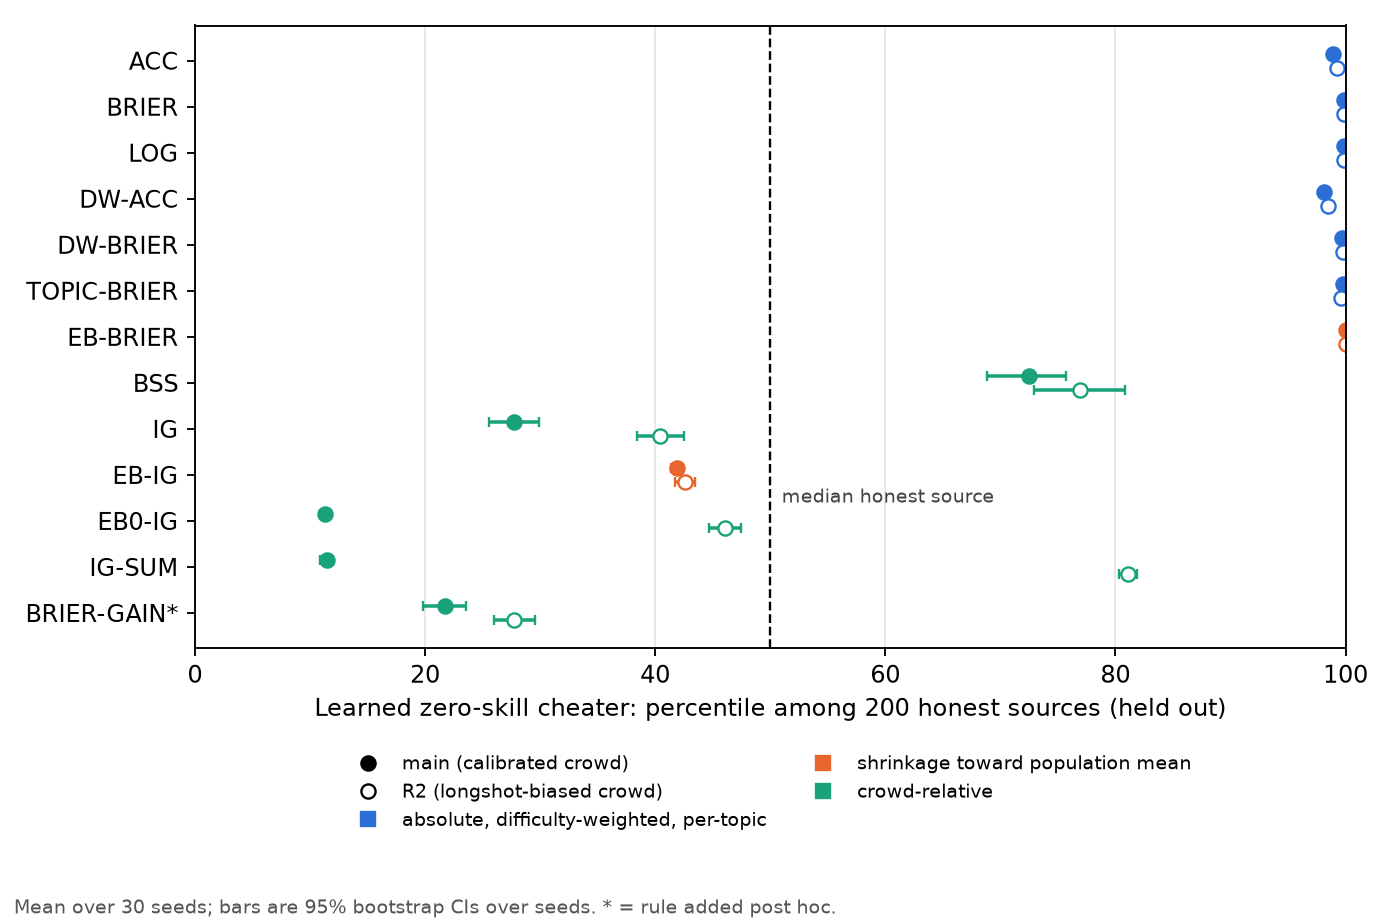
\includegraphics[width=0.5\linewidth]{figures/fig1_cheater_inflation_30seeds.png}
\caption{How far does a trained zero-skill cheater climb, by rule? Dots are mean held-out percentiles among 200 honest sources over 30 seeds. Bars are 95\% bootstrap CIs over seeds. Filled: calibrated crowd (main). Open: longshot-biased crowd (R2). The dashed line is the median honest source. * marks a rule added post hoc. Source: \file{results/E03/sim_30seeds_summary.csv}.}
\label{fig:infl}
\end{figure}



\textbf{Absolute rules fall to cherry-picking.} The learned cheater reaches the 98.9th percentile under accuracy and the 99.8th under Brier (Figure~\ref{fig:infl}; Table~\ref{tab:A1} gives CIs, seed ranges and the hand-coded comparison). Plain cherry-picking of near-certain events reaches the same ceiling. Heuristic difficulty weights ($4c(1-c)$ from the crowd prior), a coarse topic mean and shrinkage toward the mean do not help: all seven absolute, difficulty-weighted, per-topic and shrunk rules score 98 or higher. Rules that use other sources' claims do better, but still leak (next paragraph). This confirms the known selection effect \citep{sempere2021}. The pre-registered signal test passed in the pilot.

\textbf{Peer and fixed-effect rules (review round, 30 seeds).} We tested whether pairwise peer scoring or question fixed effects remove the selection gain. Copying the crowd scores only 14.2 [13.7, 14.6] under PEER and 12.6 under PEER-SUM, so the hypothesis that peer scores differ from crowd-relative scores through Jensen's inequality is not supported here. But the learned cheater reaches 46.0 [43.7, 48.3] (PEER), 46.8 (PEER-SUM) and 43.2 [41.6, 44.8] (FE-BRIER), and about 52.5 under R1 for the peer rules. That is near the median and far above IG-SUM's 11.5, so these rules are more gameable here. They are not gameable like absolute rules (98 to 100). Appendix Table~\ref{tab:newrules} gives all conditions.

\textbf{The learner finds what hand-coding missed.}
\begin{itemize}\setlength{\itemsep}{1pt}\setlength{\parskip}{0pt}
\item \emph{BSS as a ratio: 72.5, against 20.2 for the best hand-coded cheat.} The learned policy makes about 11 claims, all on events where the crowd is at least 95\% sure. If every favourite wins, the source's Brier total is far below the crowd's, and the ratio is near 1. One upset costs little. The percentile is roughly the chance that all 11 favourites win. The seed spread is wide: standard deviation 9.8, range 39.2 to 89.4. BSS is the highest-variance rule. Rewriting it as a difference (BRIER-GAIN) gives 21.7.
\item \emph{Shrinkage toward the population mean: 41.9, against 23.3.} The learner makes the minimum 10 claims and roughly copies the crowd. Shrinkage hands it about the average source's information gain. Shrinking toward zero instead (EB0-IG) holds it at 11.3.
\end{itemize}

\textbf{Crowd-relative rules hold, in the main condition.} Mean information gain gives 27.8. The learner makes 10 claims on 80 to 95\% favourites and extremizes hard. This variance gamble loses in expectation but lands above the median in 33\% of test worlds. EB0-IG and IG-SUM resist every attack we ran: no hand-coded policy beats copying the crowd, and the cheater is never above the median in any test world. Copying the crowd lies inside the policy class, so a learned cheater scoring slightly below it (11.3 against 12.3 for EB0-IG, and lower with five times more search) is overfitting to its 40 training worlds, not a better defence.

\textbf{Robustness (10-seed pilot, Table~\ref{tab:A2}).} Five times more search changed no verdict. A 30-claim minimum removes most variance gambles (IG 11.6, EB0-IG 6.7) but not the BSS exploit (44.7).

\subsection{Why rules fail: three mechanisms}
\label{sec:mech}
\textbf{Mechanism 1: absolute scores reward easy picks.} A source that copies a crowd prior $c$ has an expected Brier score of $c(1-c)$. Its expected accuracy is $\max(c, 1-c)$. Both improve as claimed events get easier. On a 97\% event the expected Brier score is 0.029. On a 50\% event it is 0.25. Cherry-picking is optimal, and heuristic difficulty weights cancel when every claimed event is easy.

\textbf{Mechanism 2: ratios and mean-shrinkage break the zero-skill bound.} Let $F$ be the public information on all events (crowd priors and topics) plus the source's own randomization. A zero-skill source fixes its claim indicators $z_i$, hence its volume $N=\sum_i z_i$, and its reports $r_i$ as functions of $F$ before any outcome is revealed. With a proper score $S$ and a calibrated crowd, $\mathbb{E}[S(r_i,y_i)-S(c_i,y_i)\mid F]\le 0$ for every event. Any non-negative $F$-measurable weights $w_i$ then give a non-positive expected weighted sum, $\mathbb{E}[\sum_i w_i\,(S(r_i,y_i)-S(c_i,y_i))\mid F]\le 0$: $w_i=z_i$ for IG-SUM, and $w_i=z_i/N$ ($N>0$) for the means IG and BRIER-GAIN. Two points follow. First, the effective weights of BSS depend on the realized outcomes through its denominator, so they are not $F$-measurable and the bound does not apply. Ratio skill scores of this kind are known to be improper \citep{murphy1973,jolliffe2008}. Shrinkage toward the population mean fails differently: a source with little history receives the average source's credit. Second, the bound is on the expected score, not the expected percentile. A mean over $N=10$ claims has variance proportional to $1/N$, so a low-volume, extremized gamble lands above the honest median in some worlds. That lifts IG to 27.8 and BRIER-GAIN to 21.7, while summing (IG-SUM) and shrinkage toward zero (EB0-IG) damp low-volume variance. The bound also needs outcome-blind selection. Our cheater selects from crowd bins and topics only. With outcome-dependent stopping the means could do better.

\textbf{Mechanism 3: the bound needs a calibrated baseline.} In R2 the crowd has a predictable bias. A source with no private information can earn positive information gain by undoing it. The learned IG-SUM cheater floods, with about 990 claims, and sets $\alpha$ near the inverse of the injected bias. Every crowd-relative rule moves up (Figure~\ref{fig:infl}, open dots). Total information gain reaches 81.1, EB0-IG 46.1 and IG 40.5. Table~\ref{tab:A1} gives the other rules under R2.

\subsection{Does recalibrating the baseline close the gap?}
\label{sec:recal}
Using the protocol of Section~\ref{sec:recalmethod}, Figure~\ref{fig:recal} and Table~\ref{tab:A9} give the learned-cheater percentile under each baseline. The raw-crowd rows score only the 2,250 eligible events, so they differ slightly from Table~\ref{tab:A1}.

\begin{figure}[t]
\centering
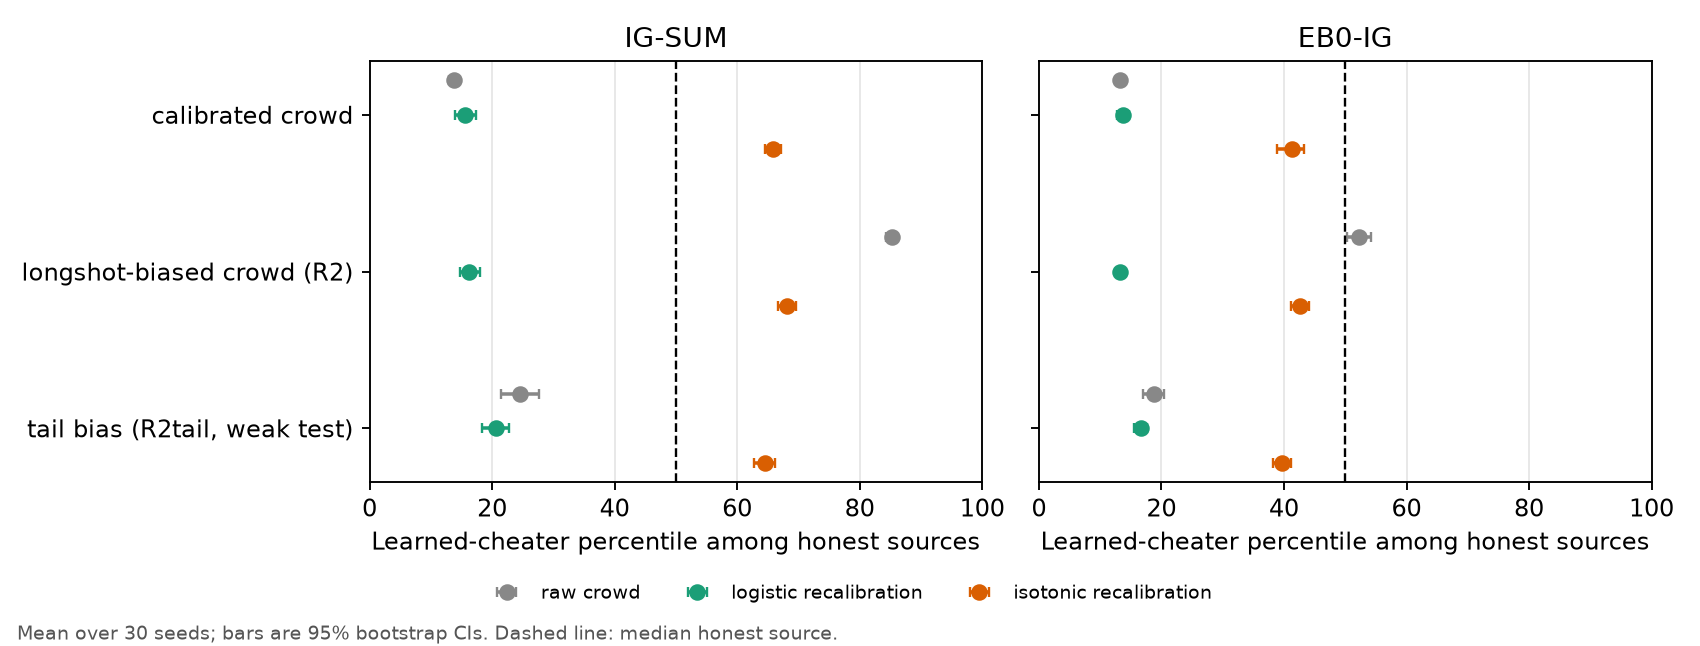
\includegraphics[width=0.58\linewidth]{figures/fig3_recalibration.png}
\caption{Does recalibration restore resistance to the learning cheater? Learned-cheater percentile for IG-SUM and EB0-IG under no, logistic and isotonic recalibration of the baseline, in three worlds. Dots are means over 30 seeds. Bars are 95\% bootstrap CIs. The dashed line is the median honest source. Source: \file{results/E03/sim_recal_summary.csv}.}
\label{fig:recal}
\end{figure}

\textbf{Logistic recalibration works in the favourable case.} Under R2, IG-SUM falls from 85.2 [84.3, 86.1] to 16.2 [14.7, 18.0], and EB0-IG from 52.3 to 13.3. All 30 seeds are below the median for IG-SUM (worst seed 31.8). The learned policy changes from about 990 claims to about 41, so the flood-and-invert strategy no longer pays. But the injected bias is exactly logistic in log-odds, so the fitted map is well specified. This is the favourable case. Under a calibrated crowd the logistic baseline costs little (IG-SUM 15.5 [14.0, 17.3] against 13.8 [12.9, 14.6]).

\textbf{Isotonic recalibration fails, even with no bias.} IG-SUM stays at 68.2 [66.6, 69.7] under R2 and reaches 65.8 [64.5, 67.1] with a calibrated crowd. The step function, fitted on at most 2,250 noisy outcomes, has a mean baseline error of 0.031 (0.032 under R2), against 0.012 for the logistic map, so the baseline is worse than the raw calibrated crowd. A cheater that floods about 980 claims and copies the published crowd earns positive summed information gain. A baseline must be calibrated in expectation, and estimation noise is exploitable by volume. The recommendation must therefore name the form of recalibration.

\textbf{BSS is not fixed.} BSS stays between 71 and 80 under every baseline, and EB-IG between 40 and 42. A ratio stays exploitable whatever the baseline.

\textbf{A misspecified distortion.} R2tail barely hurts the raw baseline (IG-SUM 24.5), so it does not stress the logistic map. We therefore tested one asymmetric distortion with the same mean baseline error as R2 (0.044): favourites are under-priced as $c=0.5+0.5(2p-1)^{2.10}$ for $p\ge0.5$. The raw baseline gives IG-SUM 92.4 [92.0, 92.8], isotonic 56.6 [53.7, 59.1] and logistic 29.2 [25.8, 32.6], with one seed at 48.1 (Appendix Table~\ref{tab:asym}). Logistic recalibration still helped, but less than in the well-specified case (16.2). This is one shape and one size only. We ran no separate hand-crafted attack on the fit, and we do not claim the recalibrated baseline is attack-proof.

\subsection{Real data: Manifold Markets}
\label{sec:manifold}
\begin{figure}[t]
\centering
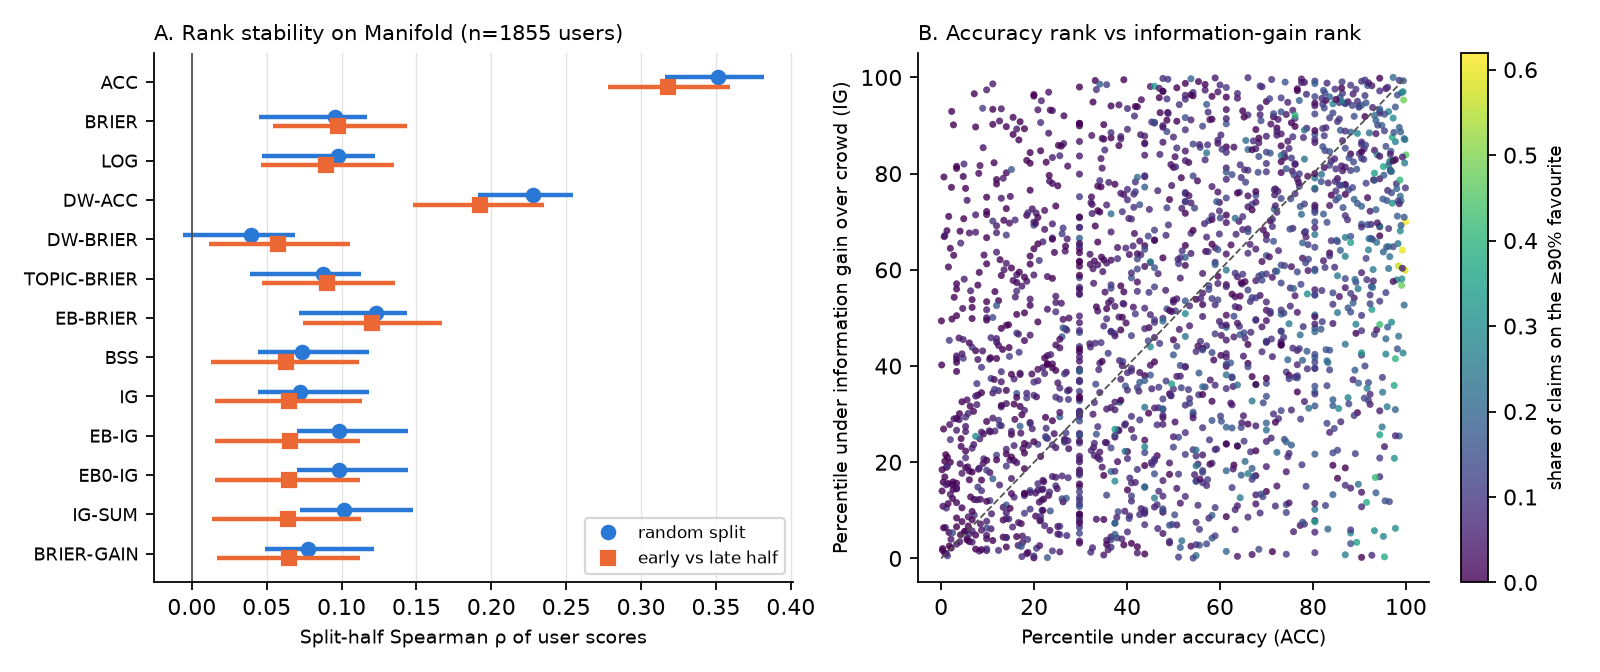
\includegraphics[width=0.64\linewidth]{figures/fig2_manifold.png}
\caption{Are real rankings stable, and do they show the gaming signature? (A) Split-half Spearman correlation of user scores by rule, 95\% bootstrap CIs over users ($n=1{,}855$). Blue: random split. Orange: first half against second half in time. (B) Each dot is a user: percentile under accuracy against percentile under information gain. Colour is the share of claims on a favourite at 90\% or higher. Source: \file{results/E03/fig2_manifold.png}.}
\label{fig:manifold}
\end{figure}

On real data, accuracy rankings reward a stable selection habit. Crowd-relative rules are too noisy to rank individuals, and recalibration did not help.

\textbf{Gaming signature.} Across users, the share of claims on a favourite at 90\% or higher correlates with accuracy percentile minus information-gain percentile at $\rho$ 0.42 [0.38, 0.45]. The signature is not universal: the top accuracy decile has a median information-gain percentile of 69.9, and 25.8\% of those users fall below the median. It strengthens with volume: 0.52 [0.47, 0.58] at 50 claims or more and 0.56 [0.39, 0.67] at 100 or more. Both accuracy and the favourite share are oriented by trade direction (the side bet on won). If accuracy is instead read from the post-bet price, the signature halves to 0.22. A bootstrap that resamples markets gives [0.32, 0.39], which does not contain the point estimate, because resampling markets changes which users are in the sample. The signature stays clearly positive either way.

\textbf{Stability is not validity.} Accuracy is the most stable rule (split-half $\rho$ 0.35 random, 0.32 early against late). The average crowd probability of the side a user bets on is stable too (early against late 0.56). It correlates 0.70 with accuracy and $-0.06$ with information gain. Accuracy ranks a habit of backing favourites.

\textbf{Higher volume helps, but not enough.} At 20 claims or more, crowd-relative rules have split-half $\rho$ of about 0.07 and cannot rank users. We raised the minimum to 50 claims (488 users) and 100 claims (112 users). Random-split $\rho$ for crowd-relative rules rises to 0.16 to 0.21 and then about 0.40, against 0.47 and 0.67 for accuracy. Early-against-late $\rho$ is lower, which is the test that matters for prediction (Table~\ref{tab:A3}). At 100 claims it is 0.15 to 0.23 for crowd-relative rules, and several CIs reach 0. These are heavy users, a selected subset. We do not claim that crowd-relative rules can rank individuals on this data. A directional information gain (which scores the side of the trade) is more stable, with early-against-late $\rho$ 0.11, 0.25 and 0.30 at 20, 50 and 100 claims, against 0.07, 0.12 and 0.18 for IG. It is closer to a direction-accuracy score than to a price-move score. Confidence intervals use all 20 random splits.

\textbf{The recalibrated baseline did worse on real data.} We scored claims in blocks 1 to 3 (126,526 claims) against a baseline recalibrated on earlier blocks. Out of sample, the recalibrated baseline had a mean $\log_2$ score of $-0.832$ (logistic) against $-0.790$ for the raw price (Table~\ref{tab:A6}). The fitted logistic slope and intercept drift across blocks (block 2 has intercept $-0.70$; block 3 has slope 0.86). The crowd's bias is not stationary. The median horizon from claim to resolution shrinks from 180 days in block 0 to 18 days in block 3, so horizon selection may add to this. The fit sets are markets whose last claim precedes the block start, a proxy for ``resolved'': 1, 3 and 42 of the 81, 261 and 469 fit markets (blocks 1 to 3) actually resolved later (9\% in block 3). So the baseline was not fitted only on already-resolved events. This leak favours recalibration, so it does not explain the negative result. Rank stability did not improve (IG early against late 0.064 raw, 0.011 logistic). The simulated fix assumes a stationary bias. We make no claim that recalibration improves real leaderboards.

\textbf{Caveats.} In an automated market maker, the post-bet price of a small bet is close to the pre-bet price ($r\approx c$). Crowd-relative scores then mostly measure bet size and liquidity, which can depress their stability. Results may not carry over to platforms where probabilities are stated directly. Play money. There is no ground-truth skill, so the data show stability and signatures, not which rule is right. The favourite share is a correlational signature, not proof of intent.

\subsection{A small check with a language-model pundit}
A language model told the rule rediscovers cherry-picking, and nothing more. This is a small supporting check, not a result. Under accuracy and Brier the pundit finds cherry-picking, with held-out percentiles of 98.8 and 99.0. Under IG, IG-SUM and BSS it stays below the median in every run (0.7, 5.2 and 13.8; Table~\ref{tab:A7}). It does not find the BSS exploit when told to optimize BSS (5.5 to 24.5), consistent with its 300-event pool, 10 to 60 claim cap and 8-candidate search. One run told to optimize accuracy (17 claims) did reach a BSS percentile of 100. A failure to find an exploit is not evidence that none exists. There are 3 to 4 held-out runs per rule and one model family (Table~\ref{tab:A7} gives each run). One run of gemma-4-31b-it under IG returned an invalid claim set twice, so that cell has one run.

\subsection{Recommended rule and audit checklist}
No audited rule both holds the cheater near the bottom and recovers honest skill best. Among the cheater-resistant rules, EB0-IG is the better compromise. Both statements hold in simulation and, for recalibration, for a stationary bias.
\begin{enumerate}\setlength{\itemsep}{1pt}\setlength{\parskip}{0pt}
\item \textbf{Use a difference of proper scores against a baseline. Never use a ratio.} BSS gave 72.5 and stays at 71 to 80 under every baseline. Its difference form gave 21.7. We do not recommend BSS.
\item \textbf{Aggregate by sum, or shrink toward zero skill. Never shrink toward the population mean.} IG-SUM and EB0-IG gave 11.5 and 11.3. EB-IG gave 41.9. IG-SUM ranks honest sources by volume (Spearman 0.74) more than by skill (0.36). EB0-IG is less volume-driven (0.61) and recovers more skill (0.45), so we prefer it. Peer rules recover skill best (0.60 to 0.66, volume near 0) but let the cheater reach 43 to 47.
\item \textbf{Set a minimum volume.} A 30-claim floor cut IG from 27.3 to 11.6 (10-seed pilot, Table~\ref{tab:A2}).
\item \textbf{Time-stamp the baseline before the claim.} The bound needs a pre-claim baseline.
\item \textbf{If the crowd baseline may be biased, recalibrate it with a low-variance parametric map, such as a two-parameter logistic fit on past resolved events. Do not use isotonic regression.} Logistic recalibration cut IG-SUM from 85.2 to 16.2 under a logistic bias. Isotonic recalibration left it at 68.2.
\item \textbf{Test the recalibration out of sample on your own data before adopting it.} On Manifold the recalibrated baseline was worse than the raw price. If the bias drifts, a past-fitted map can hurt.
\item \textbf{Check honest-skill recovery, dependence on volume and rank stability alongside cheater resistance.} In main, skill recovery is 0.26 to 0.39 for absolute rules and 0.45 to 0.66 for crowd-relative and peer rules; volume correlation is 0.74 for IG-SUM and 0.61 for EB0-IG and near 0 otherwise (Appendix Table~\ref{tab:skillvol}). On Manifold, stability is low for every rule (Section~\ref{sec:manifold}).
\end{enumerate}
\textbf{Audit checklist for platform builders.}
\begin{itemize}\setlength{\itemsep}{1pt}\setlength{\parskip}{0pt}
\item Is the score an average of per-claim differences of a proper score? A ratio is an exploit.
\item What does a source with no history receive? If the population average, expect low-volume entry.
\item Can a source choose which claims enter its score? Then an absolute or heuristically difficulty-weighted score is gameable, and peer and fixed-effect scores still leak (43 to 47). We did not test a full item response model.
\item Is the baseline recorded before the claim, and is its calibration checked on resolved questions?
\item Has the score been attacked by a learner? Hand-coded cheats under-estimated two exploits here by 19 and 52 percentile points.
\end{itemize}

\section{Discussion and Limitations}
\textbf{What is new, and what is not.} Accuracy and Brier inflation through question selection is documented \citep{sempere2021}. We confirm it. The new parts are the learned-attacker audit, two exploits that hand-coded cheats missed, the three mechanisms, and the finding that a recalibrated baseline helps only when its form fits the bias.

\subsection*{Limitations}
\begin{itemize}\setlength{\itemsep}{1pt}\setlength{\parskip}{0pt}
\item \emph{Simulation assumptions.} Gaussian log-odds world, calibrated honest sources that pick events at random, a cheater that sees only the crowd prior and the topic.
\item \emph{The optimizer gives a lower bound.} A rule that resists here has resisted this search budget, not every cheater. BSS ranged from 39.2 to 89.4 across 30 seeds. The language-model check found less than the optimizer did.
\item \emph{Recalibration.} It is shown only for a matching (logistic) bias and a stationary one. Our tail-bias test was too mild, and the Manifold backtest was negative.
\item \emph{Reward and shrinkage constants.} We reward expected percentile, and a winner-take-all objective would favour variance more. The empirical-Bayes variance estimate hit its floor (complete pooling) in 40\% of Brier worlds and 8\% of IG worlds. This is not the cause of EB-BRIER at 100.0: it is 100.0 at and above the floor, and Paule--Mandel changes nothing. The cheater floods about 300 claims, so shrinkage barely touches its better-than-mean Brier, while honest sources are shrunk heavily. EB-IG is 42.7 at the floor and 41.8 above it. EB0-IG depends on the estimator under R2 (46.1 with moments, 39.8 with Paule--Mandel).
\item \emph{Real data.} Play money, no ground-truth skill, popularity-biased markets. Crowd-relative rules are too noisy to rank individuals, even at 100 claims or more on a temporal split.
\item \emph{LLM check.} 3 to 4 held-out runs per rule, one model family, a small pool.
\end{itemize}
\textbf{Dual use and future work.} The learned policies are recipes for gaming scores. We report each attack beside a rule that resists it and hash user ids (Appendix~A). Future work: a cheater with per-event features, a stronger misspecified bias, a direct attack on the recalibration fit, a drift-tracking baseline, Metaculus data and a GRPO-trained pundit (not claimed here). Further limitations are in Appendix~A.

\section{Conclusion}
A trained zero-skill cheater reaches the top of accuracy and Brier leaderboards in simulation, confirming a known selection effect. It also finds two exploits that ten hand-coded cheats missed: the Brier skill score as a ratio, and shrinkage toward the population mean. Summed crowd-relative information gain, and shrinkage toward zero skill, resist every attack we ran until the crowd baseline is predictably biased, but they rank honest sources more by volume than by skill, and peer rules that recover skill best are more gameable. A logistic recalibration restores resistance in simulation, but only because the injected bias is logistic. An isotonic recalibration fails, and on Manifold a recalibrated baseline did worse than the raw price. Platform builders should attack their own scores with a learner before adopting them.

\section*{Code and Data}
\begin{itemize}\setlength{\itemsep}{1pt}\setlength{\parskip}{0pt}
\item Code: \url{github.com/benhoangquan/ai-epistemics-2026} \authorsnote{confirm the repository is public before submitting}
\item Data: the files under \file{results/E03/} named in the appendix captions. The raw Manifold cache is not released (user ids); the derived ledger uses hashed ids.
\end{itemize}

\section*{Author Contributions}
All authors contributed equally.
\label{endbody}

\bibliographystyle{plainnat}
\begin{thebibliography}{19}\small
\bibitem[Baron et~al.(2014)]{baron2014} Baron, J., Mellers, B. A., Tetlock, P. E., Stone, E. and Ungar, L. H. (2014). Two reasons to make aggregated probability forecasts more extreme. \emph{Decision Analysis} 11(2), 133--145. \url{https://pubsonline.informs.org/doi/10.1287/deca.2014.0293}
\bibitem[Br{\"o}cker and Smith(2007)]{brocker2007} Br{\"o}cker, J. and Smith, L. A. (2007). Scoring probabilistic forecasts: the importance of being proper. \emph{Weather and Forecasting} 22(2), 382--388. \url{https://researchonline.lse.ac.uk/id/eprint/22219}
\bibitem[Jolliffe and Stephenson(2008)]{jolliffe2008} Jolliffe, I. T. and Stephenson, D. B. (2008). Proper scores for probability forecasts can never be equitable. \emph{Monthly Weather Review} 136, 1505--1510. \url{https://stormrisk.github.io/2008/jolliffe.pdf}
\bibitem[Karger et~al.(2025)]{karger2025} Karger, E. et al. (2025). ForecastBench: a dynamic benchmark of AI forecasting capabilities. ICLR 2025, arXiv:2409.19839. \url{https://arxiv.org/abs/2409.19839}
\bibitem[Merkle et~al.(2016)]{merkle2016} Merkle, E. C., Steyvers, M., Mellers, B. and Tetlock, P. E. (2016). Item response models of probability judgments: application to a geopolitical forecasting tournament. \emph{Decision} 3(1), 1--19. \url{https://repository.upenn.edu/marketing_papers/364}
\bibitem[Murphy(1973)]{murphy1973} Murphy, A. H. (1973). Hedging and skill scores for probability forecasts. \emph{Journal of Applied Meteorology} 12, 215--223. (Checked through the reference list and discussion in \citealt{jolliffe2008}; the journal page returned HTTP 403.)
\bibitem[Niculescu-Mizil and Caruana(2005)]{niculescu2005} Niculescu-Mizil, A. and Caruana, R. (2005). Predicting good probabilities with supervised learning. ICML 2005, 625--632. \url{https://mlanthology.org/icml/2005/niculescumizil2005icml-predicting}
\bibitem[Page and Clemen(2013)]{page2013} Page, L. and Clemen, R. T. (2013). Do prediction markets produce well-calibrated probability forecasts? \emph{Economic Journal} 123(568), 491--513. \url{https://ideas.repec.org/a/ecj/econjl/v123y2013i568p491-513.html}
\bibitem[Platt(1999)]{platt1999} Platt, J. C. (1999). Probabilistic outputs for support vector machines and comparisons to regularized likelihood methods. In \emph{Advances in Large Margin Classifiers}, 61--74. \url{https://users.cs.fiu.edu/~sjha/class2023/Lecture7/Slides/1999PlattScaling.pdf}
\bibitem[Satop{\"a}{\"a} et~al.(2014)]{satopaa2014} Satop{\"a}{\"a}, V. A., Baron, J., Foster, D. P., Mellers, B. A., Tetlock, P. E. and Ungar, L. H. (2014). Combining multiple probability predictions using a simple logit model. \emph{International Journal of Forecasting} 30(2), 344--356. \url{https://econpapers.repec.org/RePEc:eee:intfor:v:30:y:2014:i:2:p:344-356}
\bibitem[Turner et~al.(2014)]{turner2014} Turner, B. M., Steyvers, M., Merkle, E. C., Budescu, D. V. and Wallsten, T. S. (2014). Forecast aggregation via recalibration. \emph{Machine Learning} 95(3), 261--289. \url{https://www.doi.org/10.1007/S10994-013-5401-4}
\bibitem[Zadrozny and Elkan(2002)]{zadrozny2002} Zadrozny, B. and Elkan, C. (2002). Transforming classifier scores into accurate multiclass probability estimates. KDD 2002, 694--699. \url{https://www.cs.cornell.edu/courses/cs678/2007sp/ZadroznyElkan.pdf}
\bibitem[Gneiting and Raftery(2007)]{gneiting2007} Gneiting, T. and Raftery, A. E. (2007). Strictly proper scoring rules, prediction, and estimation. \emph{Journal of the American Statistical Association} 102(477), 359--378. DOI 10.1198/016214506000001437. \url{https://heibib.ub.uni-heidelberg.de/search/Record/1628649828}
\bibitem[Hanson(2002)]{hanson2002} Hanson, R. (2002; published 2007). Logarithmic market scoring rules for modular combinatorial information aggregation. \emph{Journal of Prediction Markets} 1(1), 3--15. \url{https://mason.gmu.edu/~rhanson/mktscore.pdf}
\bibitem[Lichtendahl and Winkler(2007)]{lichtendahl2007} Lichtendahl, K. C. Jr. and Winkler, R. L. (2007). Probability elicitation, scoring rules, and competition among forecasters. \emph{Management Science} 53(11), 1745--1755. \url{https://pubsonline.informs.org/doi/abs/10.1287/mnsc.1070.0729}
\bibitem[Rubinstein(1999)]{rubinstein1999} Rubinstein, R. (1999). The cross-entropy method for combinatorial and continuous optimization. \emph{Methodology and Computing in Applied Probability} 1, 127--190. \url{https://link.springer.com/content/pdf/10.1023/A:1010091220143.pdf}
\bibitem[Sempere and Lawsen(2021)]{sempere2021} Sempere, N. and Lawsen, A. (2021, revised 2023). Alignment problems with current forecasting platforms. arXiv:2106.11248. \url{https://arxiv.org/abs/2106.11248}
\bibitem[Witkowski et~al.(2018)]{witkowski2018} Witkowski, J., Freeman, R., Vaughan, J. W., Pennock, D. M. and Krause, A. (2018). Incentive-compatible forecasting competitions. AAAI 2018, \url{https://ojs.aaai.org/index.php/AAAI/article/view/11471}. Extended: \emph{Management Science} 69(3), 1354--1374 (2023), arXiv:2101.01816, \url{https://arxiv.org/abs/2101.01816}
\bibitem[Manifold Markets(2026)]{manifold} Manifold Markets API documentation. \url{https://docs.manifold.markets/api} (data source; endpoints \texttt{GET /v0/bets}, \texttt{GET /v0/search-markets}).
\end{thebibliography}

\appendix
\renewcommand{\thetable}{A\arabic{table}}
\renewcommand{\thefigure}{A\arabic{figure}}
\setcounter{table}{0}
\section*{Appendix}
\label{app:start}

\subsection*{A. Limitations and Dual-Use / Ethical Considerations}
\label{app:limits}
\textbf{Limitations and threats to validity.}
\begin{itemize}\setlength{\itemsep}{1pt}\setlength{\parskip}{0pt}
\item \textbf{Simulation assumptions.} The world is Gaussian in log-odds. Honest sources pick events uniformly at random and are calibrated, except in condition R1. The crowd is calibrated, except in R2. The cheater sees only the crowd prior and the topic. With richer public features, or if honest sources also select, absolute rules become noisier. The theory for crowd-relative rules is unchanged.
\item \textbf{The optimizer gives a lower bound.} The cross-entropy method finds exploits. It cannot prove that none exist. BSS ranged from 39.2 to 89.4 across 30 seeds. The EB0-IG cheater ended slightly below copy-the-crowd, so it was under-optimized. About five times more search did not change any verdict.
\item \textbf{Reward choice.} The cheater maximizes expected percentile. A winner-take-all objective would favour variance more.
\item \textbf{Empirical-Bayes constants.} The method-of-moments variance estimate hit its floor (complete pooling) in 38.5\% of worlds for Brier and 7.5\% for information gain. A better estimator could change the EB-BRIER and EB-IG numbers. It does not change EB0-IG.
\item \textbf{Population statistics.} Topic means and shrinkage constants are fit on honest sources only. One cheater among 200 barely moves them.
\item \textbf{Manifold data.} The money is play money. A bet is not a stated belief, so we use the post-bet price as the stated probability. Information gain there measures market impact, which scales with bet size. The sample is popularity-biased: it comes from the top 1,500 resolved binary markets, with 20 to 500 bettors. Topics come from a crude keyword match. There is no ground-truth skill, so the data show stability and signatures, not which rule is right. The share of claims on near-certain favourites is a correlational signature, not proof of intent. Crowd-relative rules are too noisy to rank individual users at 20 or more claims (split-half $\rho$ about 0.07).
\item \textbf{Biased baseline and recalibration.} Every crowd-relative rule fails under R2. A logistic recalibration closes the gap, but only because the injected bias is logistic. Isotonic recalibration fails. The R2tail test was too mild to stress the logistic fit. No hand-crafted attack on the fit was run beyond the learned cheater. The real-ledger backtest of recalibration was negative, because the crowd's bias drifts. The simulated fix assumes a stationary bias.
\item \textbf{LLM pundit.} 223 calls, two models from one family, 2 world pairs each, 3 to 4 held-out runs per rule, a simulated world. A third model, deepseek-v4-flash, was dropped because its reasoning used all of the 4,000-token output limit.
\item \textbf{Pilot status.} The study ran on 14 to 15 November 2026. The main and R2 conditions use 30 seeds. The other conditions use 10 (pilot) or 30 (recalibration). Exploratory conditions (R1, R2, R2tail, R3, the 5x search budget, the recalibration, the higher-volume stability, the backtest, the LLM check and the sensitivity runs) were not pre-registered. BRIER-GAIN was added post hoc.
\end{itemize}

\textbf{Dual use.} The learned policies are recipes for gaming reliability leaderboards: cherry-picking, low-volume ratio-gaming, shrink-to-mean entry and baseline recalibration with flooding. We mitigate this in four ways.
\begin{enumerate}\setlength{\itemsep}{1pt}\setlength{\parskip}{0pt}
\item We report each attack together with a rule that resists it, which favours defenders.
\item The attacks are simple and use only public information (the crowd prior and the topic). They need no access to a platform's internals.
\item We publish no per-user labels. Manifold user ids are hashed in the derived ledger, and the gaming signature is reported only as an aggregate.
\item We do not name or accuse any individual user or account.
\end{enumerate}
A platform that adopts a rule from this paper should still test it with a learned attacker. A rule that passes our audit is not proven safe.

\textbf{Ethical considerations.} The data are public Manifold Markets API responses, collected at no more than about 3 requests per second, below the documented limit of 500 per minute per IP. We did not use tokens or private data. We store the raw cache locally and do not release it, because it contains Manifold user ids. No human subjects were recruited and no personal data beyond public pseudonymous bet histories were used.

\subsection*{B. Disclosure of prior work}
All code in this project was written during the sprint, on 14 to 15 November 2026. No code from before the sprint is used. The swarm-alignment-2026 repository is not used.

\subsection*{C. Extra tables}

\begin{table}[!ht]
\centering\small
\caption{The 16 rules audited. Higher is better for every rule. $^\dagger$Added in the review round. *Rule added after the first main run showed BSS inflated; labelled post hoc (the asterisk marks it in every table and figure). $^\dagger$Rules added in the review round (Appendix Table~\ref{tab:newrules}). Exact formulas: Appendix~D.}
\label{tab:rules}
\begin{tabular}{@{}lll@{}}
\toprule
id & rule & family \\
\midrule
ACC & Accuracy & absolute \\
BRIER & Negative mean Brier & absolute \\
LOG & Mean log score in bits & absolute \\
DW-ACC & Accuracy weighted by $4c(1-c)$, $c$ = crowd prior & difficulty-weighted \\
DW-BRIER & Negative Brier, same weights & difficulty-weighted \\
TOPIC-BRIER & Topic mean Brier minus own Brier & per-topic \\
EB-BRIER & Brier, shrunk toward the population mean & shrinkage \\
BSS & 1 minus (source Brier total / crowd Brier total) & crowd-relative \\
IG & Mean of log score of source minus log score of crowd & crowd-relative \\
EB-IG & IG with shrinkage toward the population mean & crowd-relative \\
EB0-IG & IG with shrinkage toward zero (the zero-skill baseline) & crowd-relative \\
IG-SUM & Total information gain over all claims & crowd-relative \\
BRIER-GAIN* & Mean of Brier(crowd) minus Brier(source) & crowd-relative \\
PEER$^\dagger$ & Mean of log score minus the honest peers' mean log score on the same event & peer \\
PEER-SUM$^\dagger$ & Sum of the same & peer \\
FE-BRIER$^\dagger$ & Minus the source effect in a two-way (source, event) fixed-effects fit of Brier & fixed effects \\
\bottomrule
\end{tabular}
\end{table}

\begin{table}[!ht]
\centering\footnotesize
\caption{Learned-cheater percentile for the 13 original rules, 30 seeds, main and R2. Mean [95\% CI over seeds], seed range. Hand-coded and copy-the-crowd columns are from the 10-seed pilot. Source: \file{results/E03/sim_30seeds_summary.csv}, \file{sim_summary.csv}. * Post hoc rule.}
\label{tab:A1}
\resizebox{\linewidth}{!}{%
\begin{tabular}{@{}lcccccc@{}}
\toprule
rule & main, 30 seeds & main seed range & R2, 30 seeds & R2 seed range & best hand-coded, main, 10 seeds & copy the crowd, main \\
\midrule
ACC & 98.9 [98.8, 99.0] & 97.9 to 99.4 & 99.2 [99.2, 99.3] & 98.9 to 99.6 & cherry+extremize (99.1) & 32.6 \\
BRIER & 99.8 [99.8, 99.9] & 99.4 to 99.9 & 99.9 [99.8, 99.9] & 99.5 to 100.0 & cherry-pick (99.8) & 29.5 \\
LOG & 99.9 [99.8, 99.9] & 99.5 to 100.0 & 99.9 [99.8, 99.9] & 98.4 to 100.0 & cherry-pick (99.8) & 29.2 \\
DW-ACC & 98.2 [97.9, 98.4] & 96.2 to 99.2 & 98.5 [98.2, 98.7] & 95.0 to 99.1 & cherry+extremize (99.0) & 29.6 \\
DW-BRIER & 99.7 [99.6, 99.8] & 98.0 to 100.0 & 99.8 [99.8, 99.9] & 99.2 to 100.0 & cherry-pick (99.9) & 24.3 \\
TOPIC-BRIER & 99.8 [99.7, 99.8] & 99.1 to 100.0 & 99.6 [99.5, 99.8] & 98.6 to 100.0 & cherry-pick (99.3) & 29.3 \\
EB-BRIER & 100.0 [100.0, 100.0] & 100.0 to 100.0 & 100.0 [100.0, 100.0] & 100.0 to 100.0 & cherry-pick (99.9) & 27.2 \\
BSS & 72.5 [68.9, 75.7] & 39.2 to 89.4 & 76.9 [73.0, 80.8] & 54.1 to 93.7 & low-vol-gamble (20.2) & 13.1 \\
IG & 27.8 [25.6, 29.9] & 16.5 to 40.3 & 40.5 [38.5, 42.5] & 29.9 to 51.3 & low-vol-gamble (17.3) & 12.3 \\
EB-IG & 41.9 [41.4, 42.3] & 38.4 to 44.3 & 42.6 [41.7, 43.4] & 36.4 to 48.4 & low-vol-gamble (23.3) & 8.1 \\
EB0-IG & 11.3 [10.9, 11.8] & 8.7 to 13.5 & 46.1 [44.7, 47.5] & 38.1 to 56.5 & copy-crowd (12.3) & 12.3 \\
IG-SUM & 11.5 [10.9, 11.9] & 6.9 to 13.6 & 81.1 [80.3, 81.8] & 75.5 to 84.7 & copy-crowd (12.3) & 12.3 \\
BRIER-GAIN* & 21.7 [19.9, 23.5] & 12.3 to 30.2 & 27.8 [26.0, 29.6] & 19.0 to 41.0 & low-vol-gamble (17.3) & 13.1 \\
\bottomrule
\end{tabular}}
\end{table}

\begin{table}[!ht]
\centering\footnotesize
\caption{Robustness: learned-cheater percentile by condition (10-seed pilot). Mean [95\% CI over 10 seeds]. Source: \file{results/E03/sim_summary.csv}, conditions main, R1, R2, R3, main\_strong. R1: miscalibrated honest sources. R2: crowd with longshot bias. R3: minimum 30 claims. Strong: about 5x the search budget.}
\label{tab:A2}
\resizebox{\linewidth}{!}{%
\begin{tabular}{@{}lccccc@{}}
\toprule
rule & main & R1 & R2 & R3 & main, strong search \\
\midrule
ACC & 98.9 [98.7, 99.0] & 98.9 [98.8, 99.0] & 99.3 [99.2, 99.4] & 100.0 [99.9, 100.0] & 98.8 [98.4, 99.0] \\
BRIER & 99.8 [99.7, 99.9] & 99.7 [99.6, 99.8] & 99.9 [99.9, 99.9] & 100.0 [100.0, 100.0] & 99.9 [99.8, 99.9] \\
BSS & 69.4 [59.9, 77.5] & 73.8 [70.5, 77.2] & 74.5 [67.0, 81.5] & 44.7 [39.8, 48.9] & 73.8 [69.2, 78.4] \\
IG & 27.3 [23.6, 30.9] & 28.3 [25.5, 31.4] & 40.2 [37.1, 43.7] & 11.6 [10.2, 13.2] & 25.3 [22.1, 28.5] \\
EB-IG & 41.2 [40.4, 41.9] & 43.2 [42.4, 44.1] & 42.8 [41.4, 44.3] & 32.3 [31.7, 32.8] & 42.0 [41.4, 42.5] \\
EB0-IG & 10.8 [10.2, 11.5] & 20.3 [19.6, 21.0] & 46.0 [43.9, 48.0] & 6.7 [6.1, 7.2] & 9.2 [7.5, 10.8] \\
IG-SUM & 10.7 [9.6, 11.7] & 20.1 [19.5, 20.7] & 81.9 [80.7, 83.0] & 7.0 [6.6, 7.3] & 10.8 [10.0, 11.5] \\
BRIER-GAIN* & 19.9 [17.4, 22.4] & 21.3 [18.2, 24.5] & 28.1 [25.2, 31.6] & 9.7 [8.8, 10.7] & 19.6 [17.5, 21.5] \\
\bottomrule
\end{tabular}}
\end{table}

\begin{table}[!ht]
\centering\footnotesize
\caption{Split-half rank stability on Manifold, the 13 original rules, three minimum claim counts. Spearman $\rho$ [95\% bootstrap CI over users]. Sources: \file{results/E03/real_stability_main.csv}, \file{real_min50/real_stability_main.csv}, \file{real_min100/real_stability_main.csv}. The random-split CI here is bootstrapped over 5 of the 20 splits (a compute shortcut in the original code, not a statistical choice); Table~\ref{tab:stab2} gives CIs over all 20 splits, which are similar or slightly narrower. Heavy users are a selected subset. At minimum 100 claims the early-against-late CIs for IG, EB-IG, EB0-IG and IG-SUM reach 0.}
\label{tab:A3}
\resizebox{\linewidth}{!}{%
\begin{tabular}{@{}lcccccc@{}}
\toprule
rule & min 20 random ($n$=1,855) & min 20 early vs late & min 50 random ($n$=488) & min 50 early vs late & min 100 random ($n$=112) & min 100 early vs late \\
\midrule
ACC & 0.35 [0.32, 0.38] & 0.32 [0.28, 0.36] & 0.47 [0.42, 0.52] & 0.46 [0.39, 0.53] & 0.67 [0.57, 0.76] & 0.63 [0.48, 0.73] \\
DW-ACC & 0.23 [0.19, 0.25] & 0.19 [0.15, 0.23] & 0.33 [0.28, 0.39] & 0.32 [0.23, 0.40] & 0.54 [0.42, 0.65] & 0.52 [0.36, 0.64] \\
BRIER & 0.10 [0.04, 0.12] & 0.10 [0.05, 0.14] & 0.18 [0.11, 0.24] & 0.18 [0.10, 0.27] & 0.35 [0.15, 0.46] & 0.34 [0.15, 0.52] \\
LOG & 0.10 [0.05, 0.12] & 0.09 [0.05, 0.14] & 0.18 [0.11, 0.24] & 0.18 [0.09, 0.26] & 0.33 [0.13, 0.44] & 0.32 [0.13, 0.49] \\
DW-BRIER & 0.04 [-0.01, 0.07] & 0.06 [0.01, 0.10] & 0.10 [0.03, 0.17] & 0.10 [0.02, 0.18] & 0.29 [0.10, 0.38] & 0.23 [0.06, 0.40] \\
TOPIC-BRIER & 0.09 [0.04, 0.11] & 0.09 [0.05, 0.14] & 0.16 [0.09, 0.23] & 0.17 [0.09, 0.26] & 0.33 [0.13, 0.45] & 0.32 [0.14, 0.51] \\
EB-BRIER & 0.12 [0.07, 0.14] & 0.12 [0.07, 0.17] & 0.20 [0.12, 0.27] & 0.18 [0.10, 0.27] & 0.37 [0.16, 0.47] & 0.35 [0.15, 0.53] \\
BSS & 0.07 [0.04, 0.12] & 0.06 [0.01, 0.11] & 0.16 [0.10, 0.24] & 0.10 [0.01, 0.19] & 0.39 [0.25, 0.53] & 0.22 [0.05, 0.39] \\
IG & 0.07 [0.04, 0.12] & 0.07 [0.02, 0.11] & 0.18 [0.11, 0.26] & 0.12 [0.02, 0.20] & 0.39 [0.23, 0.53] & 0.18 [0.00, 0.37] \\
EB-IG & 0.10 [0.07, 0.14] & 0.07 [0.01, 0.11] & 0.20 [0.13, 0.28] & 0.11 [0.01, 0.20] & 0.39 [0.23, 0.52] & 0.16 [-0.02, 0.36] \\
EB0-IG & 0.10 [0.07, 0.14] & 0.07 [0.01, 0.11] & 0.20 [0.14, 0.28] & 0.11 [0.01, 0.20] & 0.40 [0.24, 0.53] & 0.17 [-0.02, 0.35] \\
IG-SUM & 0.10 [0.07, 0.15] & 0.06 [0.01, 0.11] & 0.21 [0.14, 0.28] & 0.11 [0.01, 0.20] & 0.41 [0.24, 0.53] & 0.15 [-0.04, 0.35] \\
BRIER-GAIN* & 0.08 [0.05, 0.12] & 0.07 [0.02, 0.11] & 0.17 [0.11, 0.25] & 0.11 [0.01, 0.19] & 0.40 [0.25, 0.53] & 0.23 [0.05, 0.40] \\
\bottomrule
\end{tabular}}
\end{table}

\begin{table}[!ht]
\centering\small
\caption{Transfer, selected rows (10-seed pilot). Percentile under each scoring rule for a cheater trained on a different rule. Source: \file{results/E03/sim_transfer_main.csv}.}
\label{tab:A4}
\begin{tabular}{@{}lcccccc@{}}
\toprule
trained on & ACC & BRIER & BSS & IG & EB0-IG & IG-SUM \\
\midrule
ACC & 98.9 & 98.8 & 35.9 & 13.3 & 9.9 & 9.7 \\
BSS & 95.3 & 91.9 & 69.4 & 18.3 & 12.2 & 12.1 \\
\bottomrule
\end{tabular}
\end{table}

\begin{table}[!ht]
\centering\small
\caption{Learned policies and baseline error under recalibration (R2, IG-SUM). Source: \file{results/E03/sim_recal_policies.csv} (median over seeds) and \file{sim_recal_summary.csv}, column \texttt{cal\_err\_baseline} (mean absolute error of the baseline against the true probability). 30 seeds. $\alpha$ multiplies the logit of the published, uncalibrated crowd prior (not of the baseline), which is why it stays near the inverse of the injected bias ($1/0.75=1.33$) under recalibration.}
\label{tab:A5}
\begin{tabular}{@{}lccc@{}}
\toprule
baseline & claims & $\alpha$ & baseline error \\
\midrule
raw crowd & 990.9 & 1.30 & 0.044 \\
logistic & 41.2 & 1.44 & 0.012 \\
isotonic & 983.5 & 1.34 & 0.032 \\
\bottomrule
\end{tabular}
\end{table}

\begin{table}[!ht]
\centering\small
\caption{Real-ledger backtest of a recalibrated baseline. Mean $\log_2$ score of the baseline on 126,526 eligible claims (blocks 1 to 3). Source: \file{results/E03/real_recal_summary.json}, \texttt{baseline\_mean\_log2score\_eligible\_claims}. Fitted logistic slope and intercept by block: 0.93 and $-0.07$; 0.93 and $-0.70$; 0.86 and $-0.37$.}
\label{tab:A6}
\begin{tabular}{@{}lcccc@{}}
\toprule
baseline & all blocks & block 1 & block 2 & block 3 \\
\midrule
raw price & $-0.790$ & $-0.795$ & $-0.846$ & $-0.731$ \\
logistic & $-0.832$ & $-0.783$ & $-0.940$ & $-0.774$ \\
isotonic & $-0.833$ & $-0.784$ & $-0.941$ & $-0.776$ \\
\bottomrule
\end{tabular}
\end{table}

\begin{table}[!ht]
\centering\small
\caption{LLM pundit: held-out percentile of each run (world pair 0, world pair 1), by model. Source: \file{results/E03/llm_pundit_log.csv}, rows with \texttt{stage == B\_heldout}. The cell for gemma-4-31b-it under IG has one run because the pair-1 held-out claim set was invalid twice (fewer than 10 valid claims). Pooled min to max: ACC 98.2 to 99.8; BRIER 98.5 to 99.5; IG 0.0 to 1.0; IG-SUM 0.5 to 10.0; BSS 5.5 to 24.5. No confidence intervals are given because there are only 3 to 4 runs per rule, from two models.}
\label{tab:A7}
\begin{tabular}{@{}lcc@{}}
\toprule
rule & gemma-4-31b-it & gemma-4-26b-a4b-it \\
\midrule
ACC & 98.5, 98.2 & 98.5, 99.8 \\
BRIER & 99.5, 99.0 & 98.5, 99.0 \\
IG & 1.0 & 1.0, 0.0 \\
IG-SUM & 3.0, 7.5 & 10.0, 0.5 \\
BSS & 16.0, 9.0 & 5.5, 24.5 \\
\bottomrule
\end{tabular}
\end{table}



\begin{table}[!ht]
\centering\small
\caption{Learned-cheater percentile under recalibrated baselines. Mean [95\% CI over 30 seeds]. R2tail is a weak test (see text). The raw-crowd rows score only the 2,250 eligible events, so they differ slightly from Table~\ref{tab:A1}. Table~\ref{tab:A9} is the only table with all baselines for BSS; it does not duplicate Table~\ref{tab:A2}.}
\label{tab:A9}
\begin{tabular}{@{}llccc@{}}
\toprule
world & baseline & IG-SUM & EB0-IG & BSS \\
\midrule
main (calibrated) & raw & 13.8 [12.9, 14.6] & 13.3 [12.7, 13.9] & 72.3 [67.5, 76.7] \\
main (calibrated) & logistic & 15.5 [14.0, 17.3] & 13.7 [12.8, 14.8] & 73.5 [69.2, 77.3] \\
main (calibrated) & isotonic & 65.8 [64.5, 67.1] & 41.2 [38.9, 43.3] & 71.0 [67.2, 74.6] \\
R2 (longshot bias) & raw & 85.2 [84.3, 86.1] & 52.3 [50.3, 54.2] & 79.4 [74.6, 83.7] \\
R2 (longshot bias) & logistic & 16.2 [14.7, 18.0] & 13.3 [12.6, 14.0] & 80.1 [75.7, 84.2] \\
R2 (longshot bias) & isotonic & 68.2 [66.6, 69.7] & 42.6 [41.1, 44.0] & 79.1 [74.8, 83.1] \\
R2tail (weak test) & raw & 24.5 [21.5, 27.7] & 18.7 [17.0, 20.5] & 75.5 [70.1, 80.4] \\
R2tail (weak test) & logistic & 20.6 [18.4, 22.8] & 16.6 [15.6, 17.6] & 78.3 [73.6, 82.4] \\
R2tail (weak test) & isotonic & 64.5 [62.8, 66.2] & 39.7 [38.3, 41.2] & 78.4 [74.1, 82.3] \\
\bottomrule
\end{tabular}
\end{table}


\begin{table}[!ht]
\centering\small
\caption{Peer and fixed-effect rules (review round, 30 seeds): learned-cheater percentile, seed range, best hand-coded cheat and copy-the-crowd. Mean [95\% CI over seeds]. Source: \file{results/E03/review\_x1\_rules\_summary.csv}. Copying the crowd lands at the 10th to 23rd percentile, so the Jensen-gap hypothesis for peer scores is not supported.}
\label{tab:newrules}
\resizebox{\linewidth}{!}{%
\begin{tabular}{@{}llcccc@{}}
\toprule
rule & condition & learned cheater & seed range & best hand-coded & copy the crowd \\
\midrule
PEER & main & 46.0 [43.8, 48.3] & 32.8 to 61.3 & cherry-pick 43.3 & 14.2 [13.7, 14.6] \\
PEER & R1 & 52.5 [49.9, 55.1] & 34.4 to 66.5 & cherry-pick 52.9 & 22.5 [21.9, 23.2] \\
PEER & R2 & 49.5 [47.6, 51.4] & 40.0 to 62.5 & cherry-pick 37.2 & 10.4 [10.1, 10.8] \\
PEER-SUM & main & 46.8 [45.9, 47.7] & 39.8 to 50.3 & cherry-pick 39.8 & 12.6 [12.3, 13.0] \\
PEER-SUM & R1 & 52.7 [50.8, 54.8] & 43.5 to 71.7 & cherry-pick 55.8 & 19.2 [18.6, 20.0] \\
PEER-SUM & R2 & 47.8 [47.1, 48.4] & 43.7 to 50.9 & low-vol-gamble 34.5 & 10.3 [10.0, 10.6] \\
FE-BRIER & main & 43.2 [41.6, 44.8] & 35.5 to 51.2 & cherry-pick 48.3 & 14.6 [14.1, 15.1] \\
FE-BRIER & R1 & 47.3 [45.6, 48.9] & 36.6 to 56.7 & cherry-pick 50.8 & 18.9 [18.3, 19.6] \\
FE-BRIER & R2 & 46.3 [45.5, 47.1] & 42.0 to 50.7 & cherry-pick 47.7 & 11.4 [11.0, 11.8] \\
\bottomrule
\end{tabular}}
\end{table}

\begin{table}[!ht]
\centering\small
\caption{Honest-skill and volume recovery (review round, 30 seeds). Spearman correlation of the rule's score with true skill $k$ / with claim volume, among the 200 honest sources, by condition. Source: \file{results/E03/review\_x2\_skill\_volume.csv} (CI half-widths about 0.01 or less). IG-SUM and EB0-IG rank honest sources more by volume than by skill. The peer rules recover skill best, with volume near 0.}
\label{tab:skillvol}
\begin{tabular}{@{}lccc@{}}
\toprule
rule & main & R2 & R1 \\
\midrule
ACC & 0.26 / -0.03 & 0.27 / -0.03 & 0.27 / -0.03 \\
BRIER & 0.32 / -0.03 & 0.32 / -0.04 & 0.32 / -0.03 \\
EB-BRIER & 0.39 / 0.01 & 0.40 / 0.00 & 0.39 / 0.00 \\
BSS & 0.53 / 0.03 & 0.51 / 0.01 & 0.50 / 0.03 \\
IG & 0.54 / 0.03 & 0.54 / 0.01 & 0.48 / 0.01 \\
EB-IG & 0.60 / -0.04 & 0.60 / -0.03 & 0.54 / -0.01 \\
EB0-IG & 0.45 / 0.61 & 0.41 / 0.68 & 0.44 / 0.46 \\
IG-SUM & 0.36 / 0.74 & 0.31 / 0.80 & 0.38 / 0.57 \\
BRIER-GAIN* & 0.52 / 0.04 & 0.53 / 0.03 & 0.49 / 0.03 \\
PEER & 0.60 / -0.00 & 0.61 / -0.00 & 0.52 / -0.02 \\
PEER-SUM & 0.66 / -0.01 & 0.65 / -0.02 & 0.56 / 0.02 \\
FE-BRIER & 0.59 / -0.00 & 0.59 / -0.00 & 0.55 / -0.01 \\
\bottomrule
\end{tabular}
\end{table}

\begin{table}[!ht]
\centering\footnotesize
\caption{Recalibration under one misspecified (asymmetric) distortion, R2asym: $c=0.5+0.5(2p-1)^{\gamma}$ for $p\ge0.5$, $c=p$ otherwise, $\gamma=2.1036$ (mean baseline error 0.045, matched to R2's 0.044). Learned-cheater percentile, mean [95\% CI over 30 seeds]. Mean baseline error: raw 0.045, logistic 0.027, isotonic 0.032. One shape and one size only; IG-SUM with the logistic baseline has one seed at 48.1. * Post hoc rule. Source: \file{results/E03/review\_x4\_asym\_summary.csv}.}
\label{tab:asym}
\resizebox{\linewidth}{!}{%
\begin{tabular}{@{}lccccc@{}}
\toprule
baseline & IG-SUM & EB0-IG & IG & BRIER-GAIN* & BSS \\
\midrule
raw crowd & 92.4 [92.0, 92.8] & 65.5 [63.8, 67.0] & 39.7 [37.8, 41.7] & 41.0 [38.5, 43.5] & 77.8 [73.4, 81.8] \\
logistic & 29.2 [25.8, 32.6] & 17.4 [15.9, 18.9] & 26.1 [24.3, 27.9] & 25.9 [24.1, 27.7] & 81.7 [79.5, 83.8] \\
isotonic & 56.5 [53.7, 59.1] & 34.6 [32.4, 36.6] & 24.5 [22.9, 26.2] & 23.3 [22.0, 24.7] & 80.3 [76.9, 83.4] \\
\bottomrule
\end{tabular}}
\end{table}

\begin{table}[!ht]
\centering\scriptsize
\caption{Split-half stability with CIs over all 20 random splits (review round): random split / early against late, Spearman $\rho$ [95\% bootstrap CI over users, 300 resamples], by minimum claims ($n$ = 1,855, 488 and 112 users). ACC\_dir scores the side bet on, ACC\_price thresholds the post-bet price at 0.5, DIR-IG scores the side of the trade against the crowd with $r'=\mathrm{sigmoid}(\mathrm{logit}\,c+0.5\cdot\mathrm{direction})$. Source: \file{results/E03/real\_v3\_stability.csv}.}
\label{tab:stab2}
\resizebox{\linewidth}{!}{%
\begin{tabular}{@{}llll@{}}
\toprule
rule & $\ge$20 claims & $\ge$50 claims & $\ge$100 claims \\
\midrule
ACC\_dir & 0.35 [0.32, 0.39] / 0.32 [0.28, 0.36] & 0.47 [0.41, 0.51] / 0.46 [0.40, 0.53] & 0.65 [0.54, 0.73] / 0.63 [0.50, 0.73] \\
ACC\_price & 0.08 [0.04, 0.11] / 0.08 [0.04, 0.13] & 0.14 [0.07, 0.21] / 0.16 [0.07, 0.25] & 0.32 [0.19, 0.43] / 0.23 [0.06, 0.36] \\
BRIER & 0.10 [0.06, 0.13] / 0.10 [0.05, 0.14] & 0.18 [0.11, 0.25] / 0.18 [0.12, 0.28] & 0.34 [0.20, 0.47] / 0.34 [0.15, 0.48] \\
IG & 0.07 [0.03, 0.11] / 0.07 [0.02, 0.11] & 0.17 [0.11, 0.24] / 0.12 [0.02, 0.20] & 0.39 [0.25, 0.51] / 0.18 [-0.01, 0.36] \\
IG-SUM & 0.10 [0.07, 0.14] / 0.06 [0.02, 0.11] & 0.21 [0.14, 0.28] / 0.11 [0.02, 0.20] & 0.40 [0.26, 0.52] / 0.15 [-0.05, 0.34] \\
BSS & 0.07 [0.04, 0.11] / 0.06 [0.02, 0.11] & 0.16 [0.09, 0.23] / 0.10 [0.01, 0.18] & 0.38 [0.26, 0.49] / 0.22 [0.03, 0.39] \\
DIR-IG & 0.12 [0.09, 0.16] / 0.11 [0.06, 0.15] & 0.24 [0.19, 0.30] / 0.25 [0.18, 0.34] & 0.36 [0.22, 0.48] / 0.30 [0.13, 0.48] \\
DIR-IG-SUM & 0.17 [0.13, 0.21] / 0.15 [0.11, 0.20] & 0.27 [0.21, 0.34] / 0.26 [0.18, 0.35] & 0.39 [0.26, 0.51] / 0.30 [0.10, 0.49] \\
\bottomrule
\end{tabular}}
\end{table}

\begin{figure}[!ht]
\centering
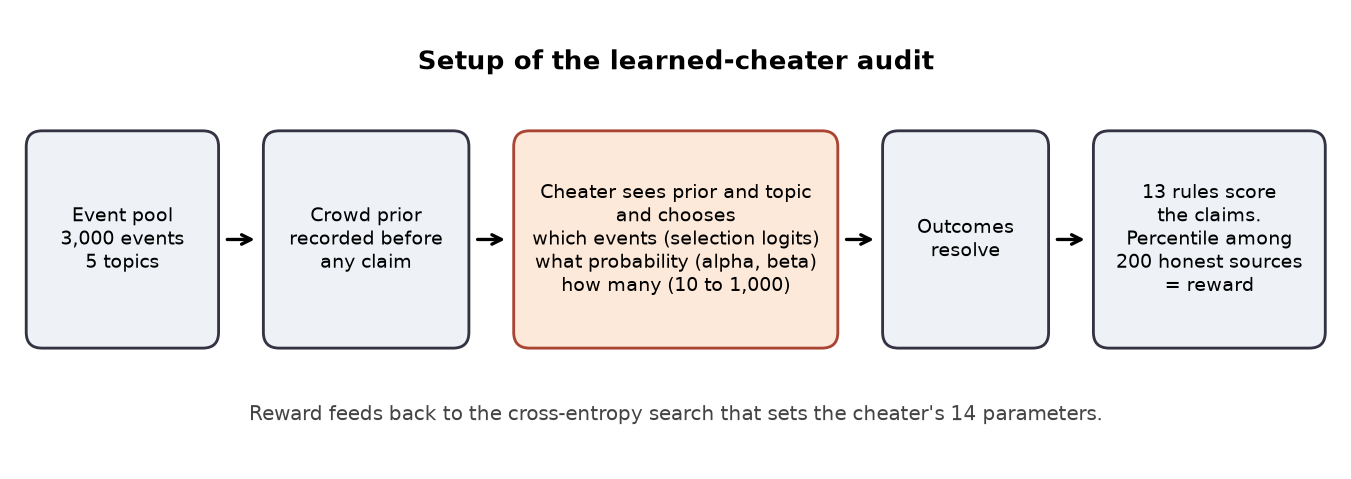
\includegraphics[width=0.55\linewidth]{figures/fig0_setup.png}
\caption{What does the cheater see, what does it choose, and where does the score come from? Schematic of one simulated world, the information available to the zero-skill cheater, its 14-parameter policy, and the score that ranks it against honest sources.}
\label{fig:setup}
\end{figure}

\subsection*{D. Specification of rules, worlds, policies and data}
\label{app:spec}
All values below are read from the code in \file{experiments/E03\_track\_record/} (\file{rules.py}, \file{sim.py}, \file{sim\_recal.py}, \file{real.py}, \file{real\_recal.py}, \file{llm\_pundit.py}). Line numbers are given in \file{review\_response.md}.

\textbf{Per-claim terms.} For a claim with stated probability $r$, crowd prior $c$ and outcome $y\in\{0,1\}$, both $r$ and $c$ are clipped to $[0.001, 0.999]$. Brier $=(r-y)^2$ and crowd Brier $=(c-y)^2$. The log score is $\log_2 r$ if $y=1$ and $\log_2(1-r)$ otherwise. Information gain is the log score of the source minus the log score of the crowd. Accuracy is 1 if $r>0.5$ and $y=1$, or $r<0.5$ and $y=0$, and 0.5 if $|r-0.5|<10^{-12}$. In the Manifold data, accuracy instead scores the side of the bet (1 if the bet side equals the outcome). The weight for DW rules is $w=4c(1-c)$.

\textbf{The 13 original rules, per source with $n$ claims.} Sums run over the source's claims.
\begin{itemize}\setlength{\itemsep}{1pt}\setlength{\parskip}{0pt}
\item ACC $=\frac1n\sum \mathrm{acc}$; BRIER $=-\frac1n\sum \mathrm{Brier}$; LOG $=\frac1n\sum \log$-score.
\item DW-ACC $=\sum w\,\mathrm{acc}/\sum w$; DW-BRIER $=-\sum w\,\mathrm{Brier}/\sum w$ (per source).
\item TOPIC-BRIER $=\frac1n\sum (\bar B_{t(i)}-\mathrm{Brier}_i)$, where $\bar B_t$ is the mean Brier of all honest claims in topic $t$ (claim-weighted, pooled over honest sources). Higher is better.
\item BSS $=1-\sum\mathrm{Brier}/\sum\mathrm{Brier}_c$. IG $=\frac1n\sum \mathrm{IG}$. IG-SUM $=\sum \mathrm{IG}$. BRIER-GAIN $=\frac1n\sum(\mathrm{Brier}_c-\mathrm{Brier})$.
\item EB-BRIER $=(n\,m+\kappa\mu)/(n+\kappa)$ with $m=-\mathrm{mean\ Brier}$. EB-IG is the same with $m=$ IG. EB0-IG $=n\,m/(n+\kappa)$ (shrinkage toward 0, using the IG constants).
\item EB constants (method of moments, over honest sources with at least 2 claims, computed separately for $-$Brier and IG): $\mu$ is the unweighted mean of source means. $s^2_w=\sum_j\sum_i (x_{ji}-m_j)^2/\sum_j(n_j-1)$. $\tau^2=\max\{\mathrm{Var}_j(m_j)-\mathrm{mean}_j(s^2_w/n_j),\,10^{-12}\}$ and $\kappa=s^2_w/\tau^2$. When the floor binds, $\kappa$ is huge and the rule pools completely (38.5\% of worlds for $-$Brier, 7.5\% for IG).
\end{itemize}
A source's percentile is the share of the 200 honest sources it beats, ties counting half. Population statistics come from the honest sources only.

\textbf{Generative model.} Topics $t_i$ are uniform on 5 topics with mean log-odds $\mu_t\in\{-2.5,-1.25,0,1.25,2.5\}$. Event $i$ has public log-odds $a_i\sim N(\mu_{t_i},1.5^2)$, difficulty $\sigma_i\sim U(0.25,2.5)$, private component $b_i\sim N(0,\sigma_i^2)$, and outcome $y_i\sim\mathrm{Bernoulli}(\mathrm{sigmoid}(a_i+b_i))$. The calibrated crowd is $c^\ast_i=\mathbb{E}[\mathrm{sigmoid}(a_i+b)\mid a_i,\sigma_i]$ by 32-point Gauss--Hermite quadrature. The published crowd is $c_i=\mathrm{sigmoid}(s\cdot\mathrm{logit}\,c^\ast_i)$ with $s=1$ (main, R1, R3) or $s=0.75$ (R2). R2tail: with $z=\mathrm{logit}\,c^\ast_i$, $z'=\mathrm{sign}(z)\,[\,|z|$ if $|z|\le2$, else $2+0.6(|z|-2)\,]$ and $c_i=\mathrm{sigmoid}(z')$. An honest source $j$ has skill $k_j\sim U(0.1,0.9)$ and volume $n_j=\mathrm{round}(\exp U(\ln n_{\min},\ln 500))$ ($n_{\min}=10$, or 30 in R3), picks events uniformly without replacement, sees $s=b_i+\varepsilon\,\sigma_i\sqrt{(1-k_j)/k_j}$ with $\varepsilon\sim N(0,1)$, and reports $\mathbb{E}[\mathrm{sigmoid}(a_i+k_js)\mid a_i,s]$, which is the Gauss--Hermite expectation with mean $a_i+k_js$ and sd $\sigma_i\sqrt{1-k_j}$. R1 reports $\mathrm{sigmoid}(\lambda_j\,\mathrm{logit}\,r)$ with $\lambda_j=\exp N(0,0.3^2)$.

\textbf{Cheater policy.} Parameters $\theta$ (14): 6 bin logits, 5 topic logits, $\alpha$, $\beta$, $\log_{10}$ volume. The 6 bins are on the folded distance $|c-0.5|$ with edges $0.1,0.2,0.3,0.4,0.45$, so bin 5 is crowd $\ge0.95$ on either side. Event weight is the bin logit plus the topic logit. The source draws $N=\mathrm{round}(10^{\theta_{14}})$ events by adding Gumbel noise to the weights and taking the top $N$, which samples without replacement and uses no outcome. The report is $r=\mathrm{sigmoid}(\alpha\,\mathrm{logit}\,c+\beta)$, clipped to $[0.001,0.999]$ when scored. Bounds: logits in $[-8,8]$, $\alpha\in[-2,8]$, $\beta\in[-4,4]$, $\log_{10}N\in[1,3]$ (lower bound $\log_{10}30$ in R3).

\textbf{Cross-entropy method.} Start at copy-the-crowd with 100 claims. Initial standard deviations: 2.0 for the 11 logits, 1.5 for $\alpha$, 1.0 for $\beta$, 0.5 for $\log_{10}N$. Each iteration draws 64 candidates (elites 12, 6 training worlds, common random numbers across candidates within a world), clips them to the bounds, and rewards the mean percentile on the target rule only. New mean is the elite mean and new standard deviation is $0.8\,\mathrm{sd}_{\rm elite}+0.2\,\mathrm{sd}_{\rm old}+0.02$. 40 iterations. The strong run uses 128 candidates, 16 elites, 8 worlds and 80 iterations. Each seed has 40 training and 20 test worlds. The test percentile averages 3 replicate draws per world.

\textbf{The 10 hand-coded cheats.} Unless stated, selection is uniform, $\alpha=1$, $\beta=0$ and 100 claims. Copy-crowd (as stated). Always-0.5 ($\alpha=0$). Cherry-pick (bin 5 only). Cherry+extremize (bin 5, $\alpha=8$). Extremize ($\alpha=3$, all events). Flood (1,000 claims). Abstain-hard (bins 3 to 5, crowd $\ge0.8$ either way). Topic-pick (topic 0, the lowest base rate). Low-volume gamble ($\alpha=3$, 10 claims). Cherry+flood (bin 5, 1,000 claims). Selected bins and topics get logit $+8$ and the others $-8$. Each is scored with 3 replicate draws on the 20 test worlds.

\textbf{Recalibration in simulation.} Events are in index order and split into 4 blocks of 750 (0-indexed, block $=\lfloor 4i/3000\rfloor$). Claims use blocks 1 to 3 (2,250 events). Block 0 is used for fitting only. The baseline for an event in block $q\ge1$ is $f_q(c)$, where $f_q$ is fitted on all events in blocks $<q$ (expanding window, event-level, 750, 1,500 and 2,250 events). Logistic: logistic regression of $y$ on $\mathrm{logit}\,c$ with $C=10^6$. Isotonic: isotonic regression of $y$ on $c$, clipped to $[0.01,0.99]$. Honest sources keep their claims on eligible events, and a source with fewer than 2 eligible claims is dropped (none were dropped on average). The cheater sees the published $c$, not the baseline.

\textbf{Review-round rules.} PEER: for each claim of a source, the log score of the source minus the mean log score of the honest peers who claimed the same event (a peer's own claim is left out for honest sources); claims on events with no peers are dropped; PEER is the mean over the remaining claims and PEER-SUM the sum. FE-BRIER: minus the source effect in a two-way (source, event) fixed-effects fit of Brier, by alternating least squares (25 sweeps, mean honest effect set to 0); the cheater's effect is solved with the honest-fitted event effects held fixed (checked against a full fit including the cheater: mean percentile differs by at most 0.1). EB-PM rules: the same empirical-Bayes rules with a Paule--Mandel estimate of the between-source variance instead of the method of moments. Asymmetric distortion R2asym: $c=0.5+0.5(2p-1)^{\gamma}$ for $p\ge0.5$ and $c=p$ otherwise, $\gamma=2.1036$, chosen so that the mean $|c-p|$ is 0.044.

\textbf{Manifold data.} Market sample: from the top 1,500 resolved binary markets, 700 sampled at random with a fixed seed, 698 kept. A bet counts if the amount is positive, it is not a redemption or an ante, the outcome is YES or NO, both prices are present, and it precedes the resolution time. A claim is a user's earliest such bet on a market. Topic rule: first match, in the order politics, sports, ai-tech, econ-finance, science-health, culture, manifold-personal, of keywords (for example ``politic'', ``election'', ``nfl'', ``openai'', ``crypto'', ``covid'', ``movie'') tested as substrings of the market's group slugs, else ``other''. Backtest blocks: the 168,701 claims are split by quartiles of claim time into 4 equal-count blocks (0-indexed). The fit for block $q$ uses claims (not markets) whose market's last observed claim precedes the start of block $q$ (a proxy for ``resolved''), expanding window, with $p_{\rm before}$ clipped to $[0.01,0.99]$ and the same logistic and isotonic settings as above. Eligible claims are blocks 1 to 3 (126,526 claims). The backtest stability analysis keeps users with at least 20 eligible claims (1,394 users, 59,587 claims), which is a different subset from the 1,855 users (83,298 claims) of the main analysis.

\section*{LLM Usage Statement}
Language models (Claude, via Claude Code) were used to write the code, run the analyses and draft the text of this paper. Other language models were the systems studied and the participants in the language-model pundit check (gemma-4-31b-it and gemma-4-26b-a4b-it). The team opened and checked each cited work. \authorsnote{confirm that you verified all claims and revised the text}

\end{document}
